\section{Einleitung}
Datenbank-Systeme finden heute in nahezu allen IT-Systemen Verwendung.
Der Optimierung von Datenbank-Anfragen kommt daher eine große Bedeutung zu.
Hierfür gibt es eine Vielzahl von Möglichkeiten, z.B. Latenz und Bandbreite der Anbindung der Datenbank, Leistungsfähigkeit des Datenbank-Servers, Anzahl der Datenbank-Anfragen in der Anwendung und diverse Caching-Meachanismen.
Hat man andere Flaschenhälse ausgeschlossen oder bereits optimiert,  gilt es die für die Performance relevanten SQL-Abfragen des Systems zu identifizieren und gezielt zu optimieren. Dies können lange laufende Abfragen sein, die z.B. bei MySQL mit der Logdatei für langsame Anfragen gezielt ermittelt werden können. Oftmals sind es aber auch viele einfache, kurze Abfragen, die jedoch zu Hunderten oder Tausenden pro Sekunde auftreten und so die Anwendung viel Zeit kosten und den Datenbank-Server belasten.
Viele RDBMS stellen mit dem SQL-Kommando EXPLAIN eine Möglichkeit zur Verfügung, mehr über die innere Arbeitsweise der Datenbank bei einer bestimmten SQL-Abfrage zu erfahren. Durch gezielte Veränderung der SQL-Abfrage oder des Datenschemas kann somit die Bearbeitung der Abfrage optimiert werden.

% Eine Semesterarbeit in diesem Bereich soll sich mit MySQL spezifischen Fragestellungen auseinander setzen. 
% Es sollen auch die theoretischen Grundlagen der zu behandelnden datenbanktheoretischen Ansätze erläutern.
Die vorliegende Arbeit bezieht sich speziell auf die Optimierung von SQL-Anfragen mittels des SQL-Kommandos EXPLAIN bei dem RDBMS MySQL.
Es soll aufgezeigt werden, wie mit dem Query Execution Plan der EXPLAIN-Ausgabe die Arbeitsweise der Datenbank besser verstanden werden kann. Darauf aufbauend wird gezeigt, wie mit zielgerichteten Änderungen des Datenbank-Schemas und der SQL-Anfragen die Geschwindigkeit der Datenbank-Anfragen erheblich gesteigert werden kann.

Grundlage dieser Seminararbeit sind die Fachbücher \cite{Bradford2011}, \cite{Sauer1998}, \cite{Schwartz2009} sowie die MySQL-Referenz-Dokumentation \cite{refman1}, \cite{refman2}, \cite{refman3}.
Nach der Literaturrecherche und Bearbeitung der relevanten Fachliteratur bestand mein Betrag darin, die wesentlichen Punkte kompakt zusammenzufassen und die Vorgehensweise der Optimierung an einigen Beispielen experimentell zu demonstrieren.

\section{Theoretische Grundlagen}
\subsection{Der physische Zugriff auf die Daten}
Daten einer DB werden in der Regel auf einer Festplatte (HDD) oder einem Flash-Laufwerk (SSD) gespeichert.
Das RDBMS nutzt dazu Funktionen des Betriebssystems auf verschiedenen Ebenen.
Dateisystem-Treiber, nimmt Lese und Schreibanforderungen für Datensätze an und gibt rechnet diese in nie durchnumerierten Blöcke des Blockgerätes um. Der Blockgeräte-Treiber liest dann die entsprenden Blöcke von der Platte oder schreibt sie dort hin.

DBMS <---> Dateisystemtreiber <---> Blockgerätetreiber <---> HDD/SSD 

Auf den verschiedenen Ebenen findet hierbei Caching statt, um die relativ langsamen Zugriffe auf den Massenspeicher (HDD oder SSD) zu vermeiden oder zumindest zu bündeln. Die Reduzierung von Massenspeicher-Zugriffen ist  daher auch eine effektive Methode der DB-Anfrage-Optimierung.

\subsection{Speicherstrukturen}
Um die Daten einer Datenbank persistent zu speichern, werden diese auf einem Massenspeicher (HDD oder SSD)  abgelegt. Auf dieses sog. Blockgerät kann immer nur in Datenblöcken fester Grösse, auch Pages oder Seiten genannt, zugegriffen werden. MySQL speichert jede Tabelle in einer eigenen Datei, für einen Zugriff auf einen bestimmten Datensatz muss daher dessen Position innerhalb der Datei bekannt sein (Record-ID, RID). Andere Datenbanken wie SAP MaxDB oder Oracle speichern alle Tabellen in einer Datei (sog. Tablespace), die vorher mit einer festen Größe angelegt werden muß, um den Speicherplatz für die Daten zu reservieren (vgl. \cite{Sauer1998}, S. 145f). Es ist auch möglich, eine ganze Partition oder ein ganzes physisches Laufwerk für den Tablespace zu verwenden, womit der Overhead des Dateisystems vermieden wird und schneller auf die Datensätze zugegriffen werden kann.

Ein Grundproblem bei Datenbanken ist es, einen bestimmten Datensatz schnell aufzufinden, denn bei grossen Tabellen ist es nicht praktikabel, dafür die gesamte Tabelle zu durchsuchen. Deswegen wurden verschiedene Algorithmen und Speicherstrukturen entwickelt, die den Zugriff auf einen Datensatz mit möglichst wenig Datenträgerzugriffen ermöglichen. Heutige Festplattenlaufwerke erlauben bei Zugriffszeiten von 10ms ca. 100 zufällige Zugriffe pro Sekunden, viele Grössenordnungen langsamer als Zugriffe im RAM. Mit dem Aufkommen erschwinglicher SSDs mit einigen 10.000 bis zu einigen 100.000 Zugriffen pro Sekunde ist das Problem etwas entschärft aber immer noch vorhanden. Im folgenden werden einige Speicherstrukturen vorgestellt, die jedoch nicht alle bei einem RDBMS implementiert sein müssen.
\subsubsection{Binärbaum}
Der Binärbaum ist einer baumartige Zeigerstruktur, bei der jeder Knoten die Daten selbst (oder einen Zeiger auf die Daten) und zwei Zeiger auf weitere Knoten oder Blätter enthält. Ein Zeiger zeigt auf einen kleinere Datensatz und ein Zeiger zeigt auf einen größeren Datensatz. Ein Knoten hat also prinzipiell folgenden Aufbau:
\begin{lstlisting}
           RID:    14
Schlüssel-Wert: München
   kleiner-RID:    34
    größer-RID:    55
\end{lstlisting}
Wird ein neuer Datensatz eingefügt, so wird dessen Schlüssel-Wert verglichen mit dem Schlüssel-Wert des Wurzel-Knotens und dann rekursiv auf der kleineren oder auf der grösseren Seite des Baumes einsortiert. So ensteht eine geordnete Struktur, welche durch Rekursion in sortierter Reihenfolge gelesen werden kann. Bei häufigen Schreibzugriffen kann es passieren, dass der Binärbaum entartet. Beispielsweise würden beim Einfügen von immer grösseren Werten die rechte Seite zu einer verketteten Liste entarten. Daher muss der Baum regelmässig neu generiert (ausbalanciert) werden, was sehr aufwendig ist. Ein anderer Nachteil ist, daß bei 1000 Datensätzen, bereits 10 Ebenen, also 10 Datenträger-Zugriffe nötig sein, bei 1 Mio. Datensätzen, sind es bereits 20 Datenträgerzugriffe, also ein Zeitaufwand von etwa 0,2 Sekunden zum Auffinden eines Datensatzes (vgl. \cite{Sauer1998}, S. 147f).
\subsubsection{B-Baum}
Im Jahre 1971 wurde das Prinzip der Binärbäume von R. Bayer und E. McCraight erheblich verbessert (vgl. \cite{Bayer1972}).
Da eine Speicherseite auf dem Datenträger in der Regel mehr Speicherplatz bietet als für einen Binärbaumknoten benötigt, kann man auch in einem Knoten mehr Datensatz und Schlüssel zu Unterknoten unterbringen als in einem Binärbaumknoten. Der Baum wird dadurch breiter und flacher, mit der Folge, dass bei vielen Datensätzen weniger Knoten durchsucht werden müssen als bei dem Binärbaum. Der Verzweigungsgrad (oder die Ordnung) wird dabei von dem Algotithmus immer optimal gehalten. Der B-Baum ist dadurch automatisch immer ausbalanciert. Seit der Veröffentlichung von Bayer und McCraight 1972 wurden das Prinzip der B-Bäume mehrfach weiter verfeinert und führte zur Entwicklung der RDBMS. Heute kommt diese Datenstruktue in praktisch allen Datenbanken zur Anwendung.\\
\begin{figure}[h]
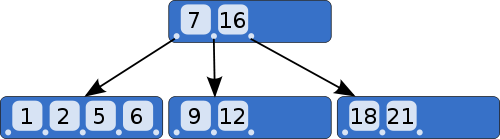
\includegraphics[width=.85\textwidth]{img/B-tree.png}
\caption{Beispiel für einen kleinen B-Baum}
\label{bbaum}
\end{figure}
\\Der Vorteil des B-Baumes degebüber dem Binärbaum ist, dass weniger Zugriffe auf den Massenspeicher notwendig sind, um zu einem Datensatz zu gelangen. Im schlechtesten Fall sind O(log(n)) Knoten zu durchsuchen. Wie auch bim Binärbaum ist beim B-Baum ein schneller Zugriff auf einen Bereich oder auf das Minimum bzw. Maximum der Daten möglich, da die Datensätze in einer definierten Ordnung abgelegt sind.

\subsubsection{Hashing}
Eine Methode um schnell auf einenDatensatz zuzugreifen ist das Hash-Verfahren. Hierbei wird der Schlüssel des Datensatzes mit einer Hash-Funktion auf eine RID abgebildet. Eine Hash-Funktion ist jedoch keine eieindeutige Abbildung, daher kann es auch zu Kollisionen kommen, mehrere Datensätze können also auf die gleiche RID abgebildet werden. In einem solchen Fall müssen dann weitere Mechanismen dafür sorgen, dass die Daten an einer anderen Stelle gespeichert und wieder aufgefunden werden können. Z.B. kann die durch nochmalige Anwendung der Hash-Funktion erfolgen oder durch einen zusätzlichen Überlaufbereich, der die Daten einfach sequentiell speichert. Damit es möglichst selten zu Kollisionen kommt und der Zugriff dadurch verlangsamt wird, muss der für die Daten reservierte Speicher gross genug gewählt werden(vgl. \cite{Sauer1998}, S. 153f).
\begin{lstlisting}[basicstyle=\ttfamily\scriptsize\singlespacing, commentstyle=,language=]
                                           +------+-----+---------+
                                           | RID  |Kdnr | Name    |
                                           |------|-----|---------|
                                           | 1000 |     |         |
  +-----+---------+                        | 1001 | 156 | Huber   |
  |Kdnr | Name    |                        | 1002 | 125 | Bauer   |
  |-----|---------|                        |  .   |     |         |
  | 123 | Bayer   |                        |  .   |     |         |
  | 124 | Schmidt |      hash(Kdnr)=RID    |  .   |     |         |
  | 125 | Bauer   |  ------------------->  |  .   |     |         |
  | 133 | Schulz  |                        |  .   |     |         |
  | 156 | Huber   |                        | 1250 | 123 | Bayer   |
  +-----+---------+                        |  .   |     |         |
                                           |  .   |     |         |
                                           |  .   |     |         |
                                           |  .   |     |         |
                                           | 2590 | 133 | Schulz  |
                                           |  .   |     |         |
                                           |  .   |     |         |
                                           | 3003 | 124 | Schmidt |
                                           +------+-----+---------+
\end{lstlisting}
Der Vorteil des Hashing besteht darin, dass die Zugriffszeit nahezu unabhänging von der Tabellengrösse ist (jedoch abhängig vom Füllgrad). In der Regel kann mit einem oder zwei Datenträgerzugriffen der Datensatz gefunden werden.
Der grösste Nachteil ist die fehlender Sortierung der Daten. Bei einem Zugriff auf einen Bereich (WHERE Name LIKE 'B%') muss die gesamte Tabelle durchsucht werden. Außerdem wird immer ein gewisser Teil des Speicherplatz verschwendet.

\subsubsection{Heap} 
Bei einem Heap (deutsch: Haufen) werden alle Datensätze einfach der Reihe nach auf dem Datenträger abgelegt. Um auf einen bestimmten Datensatz zuzugreifen, muss daher immer der gesamte Heap gelesen werden. Dies ist bei grossen Tabellen in der Regel ungünstig, kann jedoch eine Möglichkeit für kleinere Tabellen sein, die einen Umfang von einigen wenigen Speicherseiten haben, da diese komplett in den Datencache passen oder ggf. mit nur einem Datenträgerzugriff gelesen werden können.

\subsection{Abarbeitung von SQL-Ausdrücken}
Als Programmiersprache gehört SQL zu den 4GL-Sprachen. Das bedeutet, im Gegensatz zu den Programmiersprachen der 3. Generation wird nicht beschrieben WIE ein Ergebnis ermittelt werden soll sondern WELCHES Ergebnis ermittelt werden soll. Das Problem wird bei SQL also auf einem anderen semantischen Level beschrieben. Intern muss jedoch die Abfrage wieder in einen linearen Programmcode umgewandelt werden, der von der CPU bearbeitet werden kann. Dies resultiert dann zu mehr oder weniger verschachtelten Schleifen, je nach Anzahl der Tabellen, die miteinander verknüpft werden.
Sind mehrere Tabellen in die Abfrage involviert, so muss das RDBMS deren karthesische Produkt bilden um dann das Ergebnis gemäß der Bedingungen in der WHERE-Klausen einzuschränken. Wenn auf die verknüpften Spalten nicht über Indizes zugegriffen werden kann, dann müssen tatsächlich alle möglichen Kombinationen geprüft werden.

\section{MySQL-EXPLAIN}
In vielen RDBMS steht mit dem SQL-Kommando EXPLAIN ein Werkzeug zur Werfügung, um mehr darüber zu erfahren, wie die Datenbank eine bestimmte Anfrage ausführt, wie also der Query Execution Plan (QEP) ist. Das EXPLAIN-Kommando gehört jedoch nicht zum SQL-Standard und wird bei den verschiedenen RDBMS unterschiedliche Ausgaben erzeugen. Bei MySQL ist EXPLAIN sehr mächtig und gibt umfassend und datailliert Auskunft über den QEP. Hierbei muss jedoch beachtet werden, dass der QEP nicht fix ist, sondern bei jeder Anfrage vom Optimierer erneut erstellt wird (sofern die Anfrage nicht bereits aus dem Query-Cache bedient werden kann). Es gibt daher keine Garantie, dass die Anfrage immer mit dem vorher von EXPLAIN gezeigten QEP ausgeführt wird. Es empfielt sich daher, die untersuchten SQL-Anfragen von Zeit zu Zeit erneut mit EXPLAIN zu prüfen - mit Real-World-Daten.

\subsection{Umschreiben von Nicht-SELECT-Anfragen}
Vor MySQL 5.6.3 konnte EXPLAIN nur auf SELECT-Anfragen angewendet werden. \cite{refman1}
Einige Nicht-SELECT-Anfragen, wie DELETE, INSERT, REPLACE und UPDATE können jedoch in ein entsprechendes SELECT-Kommando umgeformt werden, um dieses dann mit EXPLAIN zu untersuchen. Zu beachten ist jedoch, daß schreibende Anweisungen generell aufwendiger sind als das entsprechende SELECT-Kommando, da zusätzlich zum Auffinden der Daten noch die Schreiboperation ausgeführt werden muss, ggf. kommen auch noch Aktualisierungen von Indizes hinzu.
Beispiel:
\begin{lstlisting}
  DELETE user WHERE last_login < '2012-01-01'
\end{lstlisting}
kann zu folgendem SELECT umgeschrieben werden:
\begin{lstlisting}
  SELECT id FROM user WHERE last_login < '2012-01-01'
\end{lstlisting}
Ab MySQL 5.6.3 kann EXPLAIN auf SELECT, DELETE, INSERT, REPLACE und UPDATE angewendet werden.\cite{refman1}

\subsection{Einfache SELECT-Anfragen mit einer Tabelle}
An einem Beispiel einer einfachen SELECT-Anfrage soll gezeigt werden, wie die Ausgabe einer EXPLAIN-Anweisung aufgebaut ist.
Hierzu wird zur Demonstation zuerst eine Tabelle mit einigen Daten erzeugt:
\begin{lstlisting}
mysql> CREATE TABLE words ( 
       id INT UNSIGNED AUTO_INCREMENT PRIMARY KEY, 
       word VARCHAR(60) ) ENGINE=InnoDB; 
Query OK, 0 rows affected (0,81 sec)

-- Worte aus Wörterbuch in die Tabelle laden
mysql> LOAD DATA LOCAL INFILE '/usr/share/dict/ngerman'
       INTO TABLE words (word);
Query OK, 339099 rows affected (6,58 sec)
Records: 339099  Deleted: 0  Skipped: 0  Warnings: 0
\end{lstlisting}
Es wurden also 339099 Zeilen bzw. Wörter in die Tabelle importiert, die id-Spalte hat MySQL dabei automatisch gefüllt und hochgezählt.
Nun sollen beispielhaft die fünf alphabetisch letzten Worte abgefragt werden:
\begin{lstlisting}
mysql> SELECT word FROM words ORDER BY word DESC LIMIT 5;
+-----------+
| word      |
+-----------+
| zzgl      |
| Zysten    |
| Zyste     |
| Zypressen |
| Zypresse  |
+-----------+
5 rows in set (0,20 sec)
\end{lstlisting}
Durch Voranstellen von EXPLAIN lässt sich der QEP der SELECT-Anfrage anzeigen:
\begin{lstlisting}[basicstyle=\ttfamily\scriptsize]
mysql> EXPLAIN SELECT word FROM words ORDER BY word DESC LIMIT 5;
+----+-------------+-------+------+---------------+------+---------+------+--------+----------------+
| id | select_type | table | type | possible_keys | key  | key_len | ref  | rows   | Extra          |
+----+-------------+-------+------+---------------+------+---------+------+--------+----------------+
|  1 | SIMPLE      | words | ALL  | NULL          | NULL | NULL    | NULL | 341202 | Using filesort |
+----+-------------+-------+------+---------------+------+---------+------+--------+----------------+
1 row in set (0,00 sec)
\end{lstlisting}
Wie man erkennt, wurde das EXPLAIN-Kommando schneller ausgeführt als das eigentliche SELECT.
Dies liegt daran, daß EXPLAIN nicht tatsächlich auf die Daten in der Tabelle zugreift, sondern nur aufzeigt, wie die Datenbank die Datensätze auffinden würde.

\subsection{Die Spalten der EXPLAIN-Ausgabe}
Als Ergebnis einer EXPLAIN-Anfrage liefert MySQL eine Tabelle mit festen Spalten und einer oder mehrerer Zeilen, je nach Komplexität der Anfrage. Die einzelnen Spalten haben folgende Bedeutung (vgl. \cite{refman2}, 
\cite{Schwartz2009} S. 665-676, 
\cite{Bradford2011} Pos. 2696-2906):

\textbf{id}\\*
Diese Zahl identifiziert das SELECT, zu dem die Zeile gehört. Bei einer einfachen SELECT-Abfrage steht in diesem Feld demnach immer nur die Zahl 1.

\textbf{select\_type}\\*
Die Spalte gibt an, ob es sich um ein einfaches oder komplexes SELECT handelt. Folgende Werte können hierbei auftreten:
\begin{description}
	\item[SIMPLE] einfaches SELECT, keine Unterabfragen oder UNIONS
	\item[PRIMARY] äußeres SELECT eines komplexen SELECT
	\item[SUBQUERY] SELECT in einer Unterabfrage
	\item[DERIVED] SELECT in einer Unterabfrage in der FROM-Klausel
	\item[UNION] zweites bzw. nachfolgende SELECT einer UNION
	\item[UNION RESULT] Ergebnis des UNION, wird aus temporärer Tabelle geholt
\end{description}

\textbf{table}\\*
Die Spalte Table gibt an, auf welche Tabelle zugegriffen wird. Dies kann der tatsächliche Tabellenname sein oder der Alias. Die Spalte ist von oben nach unten zu lesen, um die Join-Reihenfolge zu sehen, die der Optimierer für die Anfrage gewählt hat.
Bei komlexeren Anfragen mit abgeleiteten Tabellen und Vereinigungen können hier noch weitere Werte auftreten: <derivedN> wenn es in der FROM-Klausel eine Unterabfrage gibt, wobei N die ID der Unterabfrage ist und in den nachfolgenden Zeilen der Ausgabe zu finden ist. Bei einer Vereinigung mit UNION enthält die UNION RESULT-Zeile in der table-Spalte die IDs der Abfragen, welche vereinigt werden, und beziehen sich daher immer auf vorhergehende Zeilen der Ausgabe, z.B. <union2,4>.

\textbf{type}\\*
Wie ist der Zugriffstyp, wie wird MySQL die Zeilen in der Tabelle auffinden? Folgende Werte können hierbei auftreten (in geordneter Reihenfolge vom langsamsten zum schnellsten Zugriffstyp):
\begin{description}
\item[ALL] full Tablescan, d.h. Tabelle muss in der Regel von Anfang bis Ende durchlaufen werden, ist ein starker Indiz für weiteren Optimierungsbedarf
\item[index] wie Tablescan, aber Scannen der Tabelle erfolgt in Indexreihenfolge, eine extra Sortierung wird hierbei vermieden
\item[range] Bereichsscan, d.h. eingeschränkter Indexscan, z.B. bei BETWEEN oder > in der WHERE-Klausel
\item[ref] Indexzugriff findet statt, auch Index-Lookup genannt, Zeilen entsprechen einem Wert, nur bei einem nichteindeutigen Index, Index wird hierbei mit einem Referenzwert verglichen. Variante: ref\_or\_null
\item[eq\_ref] Index-Lookup mit eindeutigem Treffer, bei Primärschlüssel oder eindeutigem Index
\item[const,system] der Datenzugriff konnte von MySQL wegoptimiert oder in eine Konstante umgewandelt werden.
\item[NULL] Abfrage kann von MySQL bei der Optimierung aufgelöst werden, kein Zugriff auf Tabelle oder Index, z.B. Minimum einer indizierten Spalte
\end{description}

\textbf{possible\_keys}\\*
Diese Spalte gibt an, welche Indizes für die Bearbeitung der Anfrage prinzipiell zur Verfügung stehen.
Die hier stehenden Werte werden bereits in einer frühen Phase der Optimierung ermittelt, letzendlich wird in der Regel nur ein Index genutzt. Sind hier viele Indizes aufgeführt deutet das auf ein Problem hin.

\textbf{key}\\*
Die Spalte key gibt an, welcher Index der Optimierer für die Anfrage gewählt hat. Dies kann auch ein abdeckender Index sein, aus dem die Ergebniswerte gelesen werden können ohne dass die eigentliche Tabelle gelesen werden muss. Ein Wert von NULL in der Spalte key bedeutet, dass kein Index genutzt wird und ist ein starkes Indiz für einen Optimierungsbedarf.

\textbf{key\_len}\\*
wie viel Byte (Spaltenbreite) eines Index werden benutzt
welche Spalten des Index werden genutzt, von links beginnend

\textbf{ref}\\*
-welche Spalten aus früheren Tabellen werden benutzt, um in dem key-Index nachzuschlagen

\textbf{rows}\\*
Die Zahl in der Spalte rows ist eine Schätzung für die Anzahl der Zeilen, die gelesen werden müssen.
Bei Abfragen mit mehreren Tabellen bezieht sich diese Angabe pro Schleife im Nested-Loop-Join-Plan.
Die Schätzung beruht auf Statistiken kann ungenau sein. Im besten Fall steht hier eine 1.

\textbf{filtered}\\*
Die Spalte ist neu seit MySQL 5.1 und erscheint nur bei EXPLAIN EXTENDED (s.u.).
Es ist eine pessimistische Schätzung des Prozentsatzes der Zeilen, die eine Bedingung erfüllen, wie z.B. eine WHERE-Klausel oder ein JOIN mit einer anderen Tabelle.

\textbf{partitions}\\*
zeigt bei EXPLAIN PARTITIONS die verwendeten Partitionen (s.u.)

\textbf{Extra}\\*
Die Extra-Spalte enthält weitere Angaben, die nicht in die anderen Spalten passen:
\begin{description}
\item[Using Index] abdeckender Index wird genutzt, d.h. die angefragten Daten müssen nicht aus der Tabelle gelesen werden
\item[Using where] die Zeilen werden nachträglich gefiltert, d.h. für die WHERE-Bedingung wird nicht der Index genutzt
\item[Using temporary] Erstellung einer temporäre Tabelle für Sortierung 
\item[Using filesort] externe Sortierung, im RAM oder auf den Datenträger
\item[ranke checked for each record (index map: N)] kein geeigneter Index vorhanden, N ist ein Bitmap auf die Spalten in possible\_keys
\end{description}

\subsubsection{EXPLAIN EXTENDED}
Wird EXPLAIN EXTENDED anstatt von EXPLAIN verwendet, dann erscheint die zusätzliche Spalte \textbf{filtered}.
Außerdem werden weitere Informationen generiert, die mit dem nachfolgenden SQL-Kommando SHOW WARNINGS angezeigt werden können.
Eine ausführliche Beschreibung findet sich unter \cite{refman3}.

\subsubsection{EXPLAIN PARTITIONS}
Wird EXPLAIN PARTITIONS verwendet, dann zeigt zusätzlichen Spalte \textbf{partitions} die Partitionen, auf welche die Anfrage zugreift, sofern welche verfügbar sind. Diese Option ist erst seit MySQL 5.1 verfügbar.
Das Schlüsselwort EXTENDED kann nicht zusammen mit EXPLAIN PARTITIONS verwendet werden.

\subsection{Abfragen mit mehreren Tabellen}
\subsection{Optimierungsmöglichkeiten und Benchmarking}
Wichtigsten Spalten key (benutzer Index), rows (Anzahl Zeilen bearbeitet), type

QEP ist nicht fix, wird bei jeder Abfrage neu erstellt. Daher EXPLAIN einer Abfrage mit verschiedenen Beispielwerten.
Nicht mit Test-Daten testen, sondern RealWord-Daten, z.B. Backups.

ALTER TABLE users ADD INDEX

Vorsicht beim Anlegen von INDIZES: Kann bei grossen Tabellen sehr lange Dauern und blockiert in dieser Zeit die Tabelle.
Vorher Informationen über die Grösse der Tabellen holen, am besten einen Probedurchlauf auf einer Kopie machen.

Wird ein vorhandener Index bei der Anfrage nicht genutzt, obwohl er augenscheinlich genutzt werden sollte, dann kann das an veralteten Tabellen-Statistiken oder einer ungenügenden Stichprobe für die Statistiken liegen. Die Statistiken für eine Tabelle lassen sich dann mit ANALYZE TABLE Tabellenname aktualisieren.

\subsection{Visuelles EXPLAIN (graphische Werkzeuge)}

\section{Fazit und Ausblick}
% Der  Schluss  stellt  quasi  die  Abrundung  der  Arbeit  dar.  Er  beinhaltet  eine  kurze  Zusammenfassung
% der wichtigsten Ergebnisse, ein Fazit sowie einen Ausblick auf weitere Fragestellungen bzw. künftige Entwicklungen

Beschränkungen!
Optimierung wichtig
Mit Explain möglich
nicht immer exakte Angaben
Kontrolle der Optimierung mit Benchmarks nötig
möglichst bereits in den Entwicklungsprozess integrieren, und nicht erst wenn es brennt
